\item \points{2e} \textbf{Finite Differences}

To build intuition for what gradients really are, we will implement \href{https://en.wikipedia.org/wiki/Finite_difference}{finite differences} to numerically approximate gradients. This approach helps you understand the fundamental definition of derivatives and provides a valuable debugging tool for verifying analytical gradient computations.

\begin{figure}[h]
    \begin{center}
        \captionsetup{width=0.8\textwidth}
        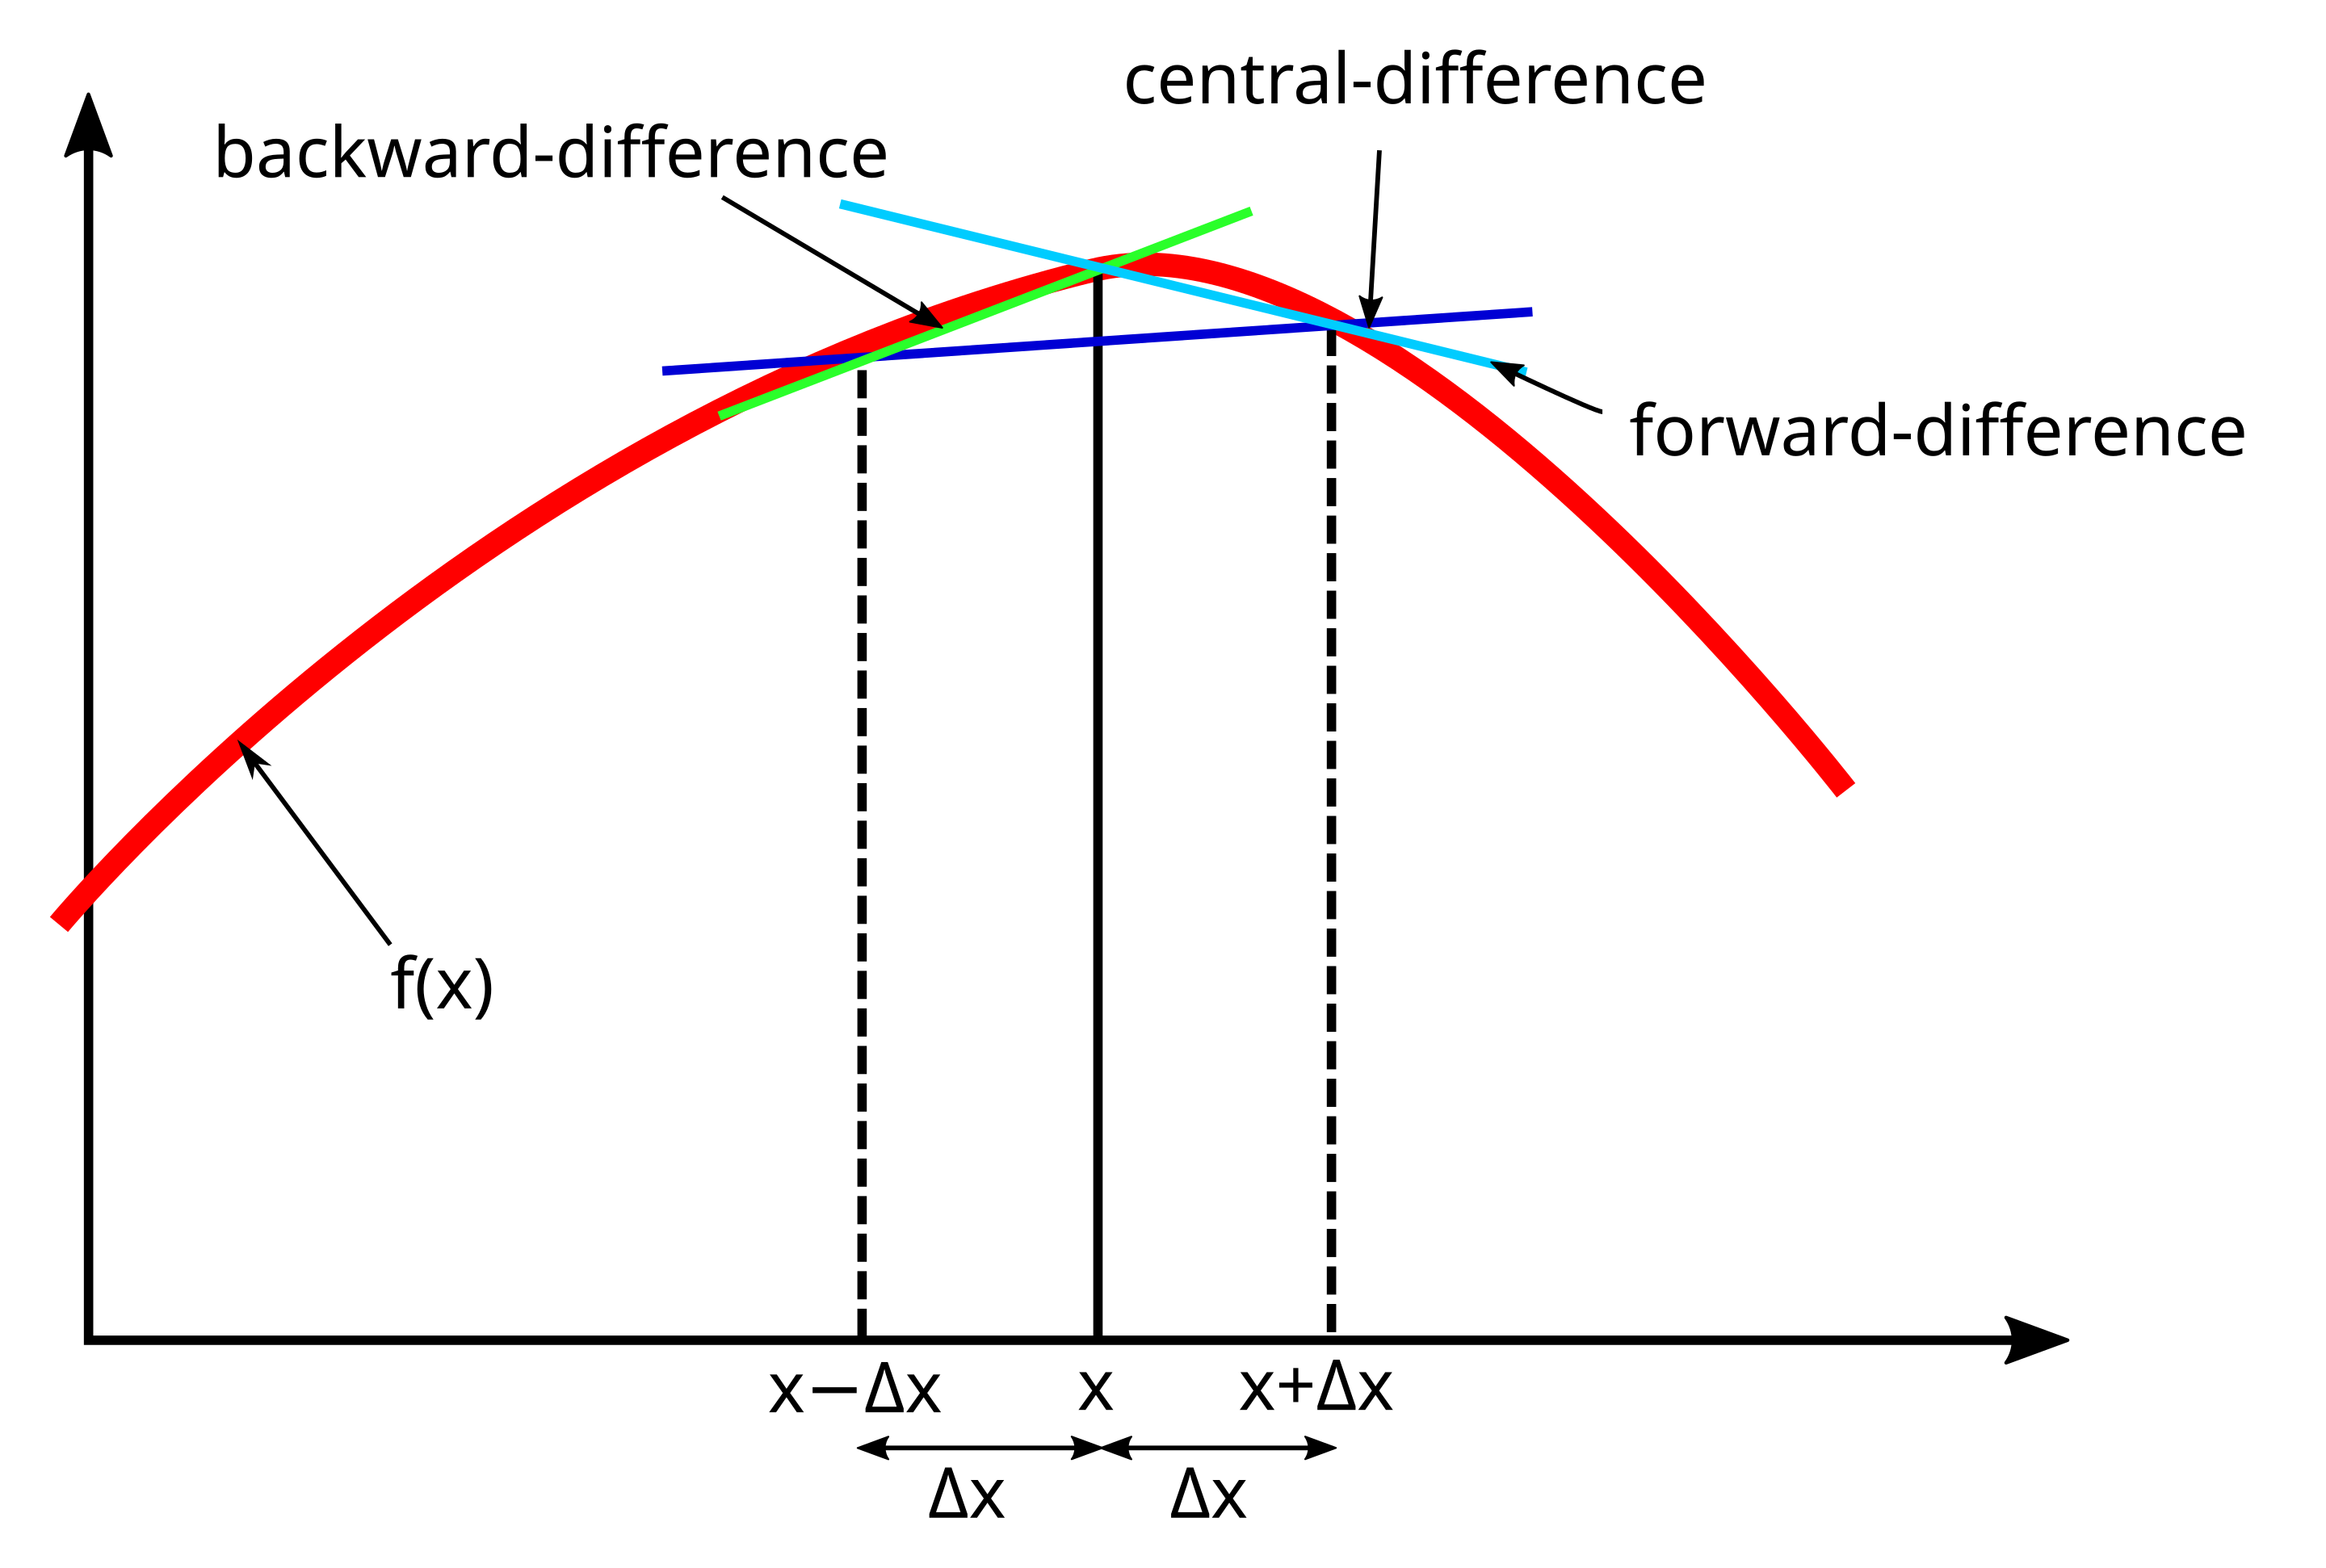
\includegraphics[width=0.7\textwidth]{images/finite-difference.png}
        \caption{Image from Wikipedia}
    \end{center}
\end{figure}

The key idea is to approximate the derivative by measuring how much the function changes when we make a small perturbation along each coordinate. The central difference formula is:
$$\frac{\partial f}{\partial w_i} \approx \frac{f(\mathbf w + \epsilon \hat{\mathbf u}_i) - f(\mathbf w - \epsilon \hat{\mathbf u}_i)}{2\epsilon}$$
where $\hat{\mathbf u}_i$ is a unit vector with 1 in the $i$-th position and 0 elsewhere, and $\epsilon$ is a small step size (like $10^{-5}$).

Think of it like checking your speedometer: if you drive a tiny distance and time how long it takes, you can estimate your speed. Similarly, if you move a tiny amount along each coordinate axis and see how the function changes, you can estimate each component of the gradient.

Now, implement two functions to compute the gradient of the least-squares objective
$f(\mathbf w) = \tfrac12\lVert A\mathbf w - \mathbf b\rVert_2^2$:
one using the analytical formula and one using finite differences for verification. Use NumPy (optionally einsum) for vectorized implementation.

\textbf{Hint: }You can use the \texttt{np.eye(d)} function to create the unit vectors.

\expect{In \texttt{submission.py}, implement \texttt{lsq\_grad(w, A, b)} (analytic gradient) and \texttt{lsq\_finite\_diff\_grad(w, A, b, epsilon=1e-5)} (central-difference gradient). The autograder will compare them on random instances.}